\lesson{7}{19.10.2023}{Монотонность функции. Критерий Коши. Замечательные пределы.}


\section{Монотонность функции}

\begin{definition}
    Пусть задана функция $f: E \subset \R \to \R$

    Функция называвется (строго, если строгий знак) монотонно возрастающей, если: 
    
    $\forall x_1, x_2 \in E: x_1 < x_2 \implies f(x_1) \leq f(x_2)$

    И (строго, если строгий знак) монотонно убывающей, если:

    $\forall x_1, x_2 \in E: x_1 < x_2 \implies f(x_1) \geq f(x_2)$
\end{definition}

\begin{remark}
    Если функция монотонна, то она либо возрастающая, либо убывающая.
\end{remark}

\begin{theorem}
    Пусть $a$ --- точка сгущения множества $E$ и $\forall x \in E: x < a$. 

    Задана функция $f: E \to \R$, $f$ --- монотонна, тогда $\exists \lim\limits_{x \to a} f(x) \in \overline{\R}$

    Если $f$ --- монотонно возрастающая, то: $$\lim\limits_{x \to a} f(x) \in \R \Leftrightarrow \exists M: \forall x \in E: f(x) \leq M \eqno(1)$$

    Если $f$ --- монотонно убывающая, то: $$\lim\limits_{x \to a} f(x) \in \R \Leftrightarrow \exists M: \forall x \in E: f(x) \geq M \eqno(2)$$

    $\newline$

    Пусть $a_1 \in \overline{\R}$ --- точка сгущения множества $E_1$ и $\forall x \in E: x > a$.

    Если $f$ --- монотонно возрастающая, то: $$\lim\limits_{x \to a} f(x) \in \R \Leftrightarrow \exists M: \forall x \in E: f(x) \geq M \eqno(3)$$

    Если $f$ --- монотонно убывающая, то: $$\lim\limits_{x \to a} f(x) \in \R \Leftrightarrow \exists M: \forall x \in E: f(x) \leq M \eqno(4)$$
\end{theorem}

\begin{proof}
    Докажем (1). Остальные доказываются аналогично.

    Пусть $\cancel{\exists} M$ из (1), тогда $\forall L > 0: \; \exists x_0 \in E: f(x_0) > L \implies \forall x > x_0: f(x) \geq f(x_0) > L \implies f(x) \underset{x \to \infty}{\to} +\infty$

    Пусть $\exists M \in \R: \forall x \in E: f(x) \leq M$. Пусть $c = \sup\{y \in \R: \exists x \in E: f(x) = y\}$. Тогда:

    $c \leq M, \forall x \in E: f(x) \leq c$. Возьмем $\forall \epsilon > 0$, тогда $\exists x_1 \in E: f(x_1) > c - \epsilon$. Имеем неравенство:

    $$c - \epsilon < f(x_1) \leq f(x) \leq c < c + \epsilon \implies f(x) \underset{x \to \infty}{\to} c, \text{ при этом } f(x) \leq \lim\limits_{x \to \infty} f(x)$$
\end{proof}

\section{Критерий Коши}

\begin{theorem} (Критерий Коши)
    Пусть есть множество $E \subset \R$, $a \in \overline{\R}$ --- точка сгущения $E$. Тогда:

    $$\exists \lim\limits_{x \to a} f(x) \Leftrightarrow \forall \epsilon > 0 \; \exists \omega(a): \forall x_1, x_2 \in \dot{\omega}(a) \cap E: |f(x_2) - f(x_1)| < \epsilon$$
\end{theorem}

\begin{proof}
    
    $\newline$
    
    \begin{itemize}
        \item[$\Rightarrow$:] Пусть $\lim\limits_{x \to a} f(x) = c \in \R$. 
        
        Тогда $\forall \epsilon > 0 \; \exists \omega(a): \forall x \in \dot{\omega}(a) \cap E: |f(x) - c| < \frac{\epsilon}{2}$

        Имеем, что $\forall x_1, x_2 \in \dot{\omega}(a) \cap E: |f(x_2) - f(x_1)| = |(f(x_2) - c) - (f(x_1) - c)| \leq |f(x_2) - c| + |f(x_1) - c| < \epsilon$

        \item[$\Leftarrow$:] Возьмем $\forall \{x_n\}_{n=1}^{\infty}, x_n \in E, x_n \neq a, x_n \underset{x \to \infty}{\to} a$. Возьмем окрестность из условия, тогда:
        
        $\exists N: \forall n > N: x_n \in \omega(a)$, значит, $\forall n, m > N, \epsilon > 0: |f(x_m) - f(x_n)| < \epsilon$ --- выполнен критерий Коши для последовательностей. А значит:

        $\exists \lim\limits_{n \to \infty} f(x_n) = c \in \R$ --- необоходимо проверить, что все последовательности сходятся к $c$.

        Предположим, что есть такая последовательность $\{x'_n\}_{n=1}^{\infty}, x'_n \in E, x'_n \neq a, x'_n \underset{x' \to \infty}{\to} a$, что $\lim\limits_{n \to \infty} f(x'_n) = c' \neq c$

        Тогда возьмем последовательность: $\begin{cases}
            \overline{x}_{2n-1} = x_n \\
            \overline{x}_{2n} = x'_n 
        \end{cases}$
        
        $\overline{x}_n \to a \overline{x}_n \in E, \overline{x}_n \neq a$, тогда по критерию Коши $\lim\limits_{n \to \infty} f(\overline{x}_{2n-1}) = \lim\limits_{n \to \infty} f(\overline{x}_{2n}) = \overline{c}$, но $\lim\limits_{n \to \infty} f(\overline{x}_{2n-1}) = \lim\limits_{n \to \infty} f(x_n) = c$ --- противоречие.
    \end{itemize}
\end{proof}

\section{Некоторые существенные неравенства}

\begin{property} (неравенство для $\ln(1 + x)$)
    Пусть $0 < x \leq \frac{1}{2}, n \in \N: \frac{1}{n+1} < x \leq \frac{1}{n}, n \geq 2$. Тогда имеем неравенства:

    \[\left(1 + \frac{1}{n}\right)^n < e < \left(1 + \frac{1}{n}\right)^{n+1}, n \geq 1 \Leftrightarrow n\ln\left(1 + \frac{1}{n}\right) < 1 < (n + 1)\ln\left(1 + \frac{1}{n}\right) \eqno(1)\]

    \[\frac{1}{n+1} < x \leq \frac{1}{n} \eqno(2)\]
    
    \[\frac{1}{x} - 1 < n \leq \frac{1}{x} \eqno(3)\]

    \[(1), (2) \implies \ln(x + 1) \leq \ln\left(1 + \frac{1}{n}\right) < \frac{1}{n} < \frac{1}{\frac{1 - x}{x}} = \frac{x}{1-x} \eqno(4)\]

    \[(1), (2), (3) \implies \ln(x + 1) > \ln\left(1 + \frac{1}{n + 1}\right) > \frac{1}{n+2} \geq \frac{1}{\frac{1}{x}+2} = \frac{x}{1 + 2x} \eqno(5)\]

    \[\text{т.е. при } 0 < x < \frac{1}{2} \text{ имеем: } \frac{x}{1+2x} < \ln(1+x) < \frac{1}{1-x} \eqno(6)\]

    Пусть теперь $-\frac{1}{3} \leq x < 0 \; (7)$, $y > 0$ и выполнено $1 + x = \frac{1}{1+y} \; (8)$

    \[(7), (8) \implies 0 < y \leq \frac{1}{2} \eqno(9)\]

    \[(6), (8), (9) \implies \ln(1 + x) = \ln\left(\frac{1}{1+y}\right) = -\ln(1 + y) < -\frac{1}{1+2y} = \frac{-\frac{x}{1+x}}{1-\frac{2x}{1+x}} = \frac{x}{1-x} \eqno(10)\]

    \[(10) \implies \ln(1 + x) < \frac{x}{1-x} \eqno(11)\]

    \[(6), (8), (9) \implies \ln(1 + x) = -\ln(1 + y) > -\frac{y}{1-y} = \frac{-\frac{x}{1+x}}{1+\frac{x}{1+x}} = \frac{x}{1+2x} \eqno(12)\]

    \[(10), (12) \implies \frac{1}{1+2x} < \ln(1 + x) < \frac{x}{1-x} \eqno(13)\]

    \[(6), (13) \implies \text{ при } -\frac{1}{3} \leq x \leq \frac{1}{2}, x \neq 0: \frac{1}{1+2x} < \ln(1 + x) < \frac{x}{1-x} \eqno(14)\]
\end{property}


\begin{remark} (2 полезных неравенства (15))
    
    при $x > 0: \frac{1}{1+2x} \leq \frac{1}{4} \Leftrightarrow x \leq \frac{1}{2}$

    при $x < 0: -\frac{1}{4} \leq \frac{x}{1-x} \Leftrightarrow -\frac{1}{4} \leq x$
\end{remark}

\begin{property} (неравенство для экспоненты)
    
    Возьмем $y = \ln(1+x)$, тогда $x = e^y - 1$:

    \[(15) \implies \text{ при } y \in \left[-\frac{1}{4}, \frac{1}{4}\right], y \neq 0 \implies x \in \left[-\frac{1}{3}, \frac{1}{2}\right], x \neq 0 \eqno(16)\]

    \[\text{ при (16: )} (13) \Leftrightarrow \frac{e^y-1}{1+2(e^y-1)} < y < \frac{e^y-1}{1-(e^y-1)} \Leftrightarrow \frac{e^y-1}{2e^y-1} < y < \frac{e^y-1}{-e^y+2} \eqno(17) \]

    \[(17) \implies e^y-1 > y(2 - e^y) \Leftrightarrow e^y(1 + y) > 1 + 2y \Leftrightarrow e^y > \frac{1+2y}{1+y} \eqno(18)\]

    \[(17) \implies e^y - 1 < y(2e^y-1) \Leftrightarrow e^y < \frac{1-y}{1-2y} \eqno(19) \]

    \[(18), (19) \text{ при } y \in \left[-\frac{1}{4}, \frac{1}{4}\right], y \neq 0: \frac{1+2y}{1+y} < e^y < \frac{1-y}{1-2y} \eqno(20)\]

    \[(20) \implies \text{ при } |x| \leq \frac{1}{3}: \frac{-2|x|}{1-2|x|} < \frac{\ln(1+x)}{x}-1<\frac{2|x|}{1-2|x|} \eqno(21)\]
\end{property}

\begin{remark}
    
    $\newline$

    $$|x| \leq \frac{1}{10}, x \neq 0 \implies \frac{2|x|}{1-2|x|} \leq \frac{1}{4} \eqno(22)$$
\end{remark}

\begin{property} (неравенство для $(1+x)^{\frac{1}{x}}$)
    \[(22) \implies (1+x)^{\frac{1}{x}} = e^{\frac{\ln(1+x)}{x}} = e^{1 + \left(\frac{\ln(1+x)}{x} - 1\right)}\]

    \[(21) \implies e^{1-\frac{2|x|}{1-2|x|}} < (1+x)^{\frac{1}{x}} < e^{1+\frac{2|x|}{1-2|x|}} \eqno(23) \]

    \[(18), (22) \implies (1+x)^{\frac{1}{x}} > e \cdot \frac{1+2\cdot\left(-\frac{2|x|}{1-2|x|}\right)}{1+\left(-\frac{2|x|}{1-2|x|}\right)} = e\cdot\frac{1-6|x|}{1-4|x|} \eqno(24)\]

    \[(18), (22), (23) \implies (1+x)^{\frac{1}{x}} < e \cdot \frac{1-\left(-\frac{2|x|}{1-2|x|}\right)}{1-2\cdot\left(-\frac{2|x|}{1-2|x|}\right)} = e\cdot\frac{1-4|x|}{1-6|x|} \eqno(25)\]

    \[(24), (25) \implies e\cdot\frac{1-6|x|}{1-4|x|}< (1+x)^{\frac{1}{x}} < e\cdot\frac{1-4|x|}{1-6|x|} \eqno(26)\]
\end{property}


\section{Замечательные пределы}

\begin{theorem} (Следствие из второго замечательного предела)
    
    $$\frac{\ln(1+x)}{x} \underset{x \to 0}{\to} 1$$
\end{theorem}


\begin{proof}
    Возьмем $f(x) = 1 - \frac{2|x|}{1-2|x|}, g(x) = , h(x) = 1 + \frac{2|x|}{1-2|x|}, \lim\limits_{x \to 0} f(x) = \lim\limits_{x \to 0} h(x) = 1$

    Из (21) имеем неравенство: $$1 -\frac{2|x|}{1-2|x|} < \frac{\ln(1+x)}{x}<1 + \frac{2|x|}{1-2|x|}$$

    По теореме о двух милиционерах получаем, что:$$\frac{\ln(1+x)}{x} \underset{x \to 0}{\to} 1$$    
\end{proof}

\begin{theorem} (Снова следствие из второго замечательного предела)
    
    $$\frac{e^x - 1}{x} \underset{x \to 0}{\to} 1$$
\end{theorem}


\begin{proof}
    
    Из (20) получаем:

    \[\frac{1+2x}{1+x} - 1 < e^x - 1< \frac{1-x}{1-2x} - 1 \implies\]

    \[\frac{x}{1+x} < e^x - 1< \frac{x}{1-2x} \implies\]

    \[1 - \frac{2|x|}{1-2|x|} < \frac{e^x - 1}{x}< 1 + \frac{2|x|}{1-2|x|} \implies\]

    \[\implies \frac{e^x - 1}{x} \underset{x \to 0}{\to} 1 \text{ --- аналогично пределу выше}\]
\end{proof}

\begin{theorem} (Второй замечательный предел)
    \[(1+x)^{\frac{1}{x}} \underset{x \to 0}{\to} e\]
\end{theorem}

\begin{proof}
    
    (23):

    \[e^{1-\frac{2|x|}{1-2|x|}} < (1+x)^{\frac{1}{x}} < e^{1+\frac{2|x|}{1-2|x|}}\]

    Значит, по теореме о двух милиционерах аналогично двум предыдущим пределам:

    \[(1+x)^{\frac{1}{x}} \underset{x \to 0}{\to} e\]
\end{proof}

\begin{theorem} (И снова следствие из второго замечательного предела)
    
    \[\frac{(1+x)^r-1}{x}  \underset{x \to 0}{\to} r\]
\end{theorem}

\begin{proof}
    Пусть $x_n \to 0, \forall n: x_n \neq 0$ и $y_n = \ln(1+x_n), y_n \neq 0$

    При $x_n \to 0, y_n \to 0$:

    \[\frac{(1+x_n)^r-1}{x_n} = \frac{e^{r\ln(1+x_n)}}{x_n} = \frac{e^{ry_n}-1}{x_n} = \frac{e^{ry_n}-1}{r \cdot y_n} \cdot r\frac{y_n}{x_n} = r\]
\end{proof}

\begin{theorem} (Первый замечательный предел)
    
    \[\lim\limits_{x \to 0} \frac{\sin x}{x} = 1\]

\end{theorem}

\begin{proof} (Простите за шакалов, я не смог засунуть сюда вектор, поэтому это всратая растровая картинка. (может исправим...))
    
    \begin{figure}[H]
        \centering
        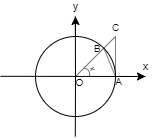
\includegraphics[width=5cm]{trig.png}
        
        
        \label{fig:1}
    \end{figure}

    Пусть дан угол $x: 0 < x < \frac{\pi}{2}$, тогда.

    $$S_{\triangle OAB} < S_{\text{сектора }OAB} < S_{\triangle AOC} \Leftrightarrow$$

    $$\Leftrightarrow \frac{1}{2} \sin x < \frac{1}{2}x < \frac{1}{2} < \tan x \implies$$

    $$\implies \sin x < x < \tan x$$

    При $1 < x \leq 1$:

    $$\cos x = \sqrt{1 - \sin^2 x} > \sqrt{1 - x^2} \geq 1 - x \implies$$

    $$\implies \sin x > x\cos x > x(1 - x)$$

    Значит получаем неравенство:

    $$1 - x < \frac{\sin x}{x} < 1$$

    При $|x| < 1, x \neq 0$ неравенство имеет вид:

    $$1 - |x| < \frac{\sin x}{x} < 1$$

    А значит по теореме о двух милиционерах:

    \[\lim\limits_{x \to 0} \frac{\sin x}{x} = 1\]
\end{proof}